\documentclass{article}
\usepackage{graphicx}
\usepackage{listings}
\usepackage{xcolor}
\usepackage{float}
\usepackage{geometry}
\usepackage{amsmath}
\geometry{a4paper, margin=1in}

\definecolor{codegreen}{rgb}{0,0.6,0}
\definecolor{codegray}{rgb}{0.5,0.5,0.5}
\definecolor{codepurple}{rgb}{0.58,0,0.82}
\definecolor{backcolour}{rgb}{0.95,0.95,0.92}

\lstdefinestyle{mystyle}{
    backgroundcolor=\color{backcolour},   
    commentstyle=\color{codegreen},
    keywordstyle=\color{magenta},
    numberstyle=\tiny\color{codegray},
    stringstyle=\color{codepurple},
    basicstyle=\ttfamily\footnotesize,
    breakatwhitespace=false,         
    breaklines=true,                 
    captionpos=b,                    
    keepspaces=true,                 
    numbers=left,                    
    numbersep=5pt,                  
    showspaces=false,                
    showstringspaces=false,
    showtabs=false,                  
    tabsize=2
}

\lstset{style=mystyle}

\title{Digital Image Processing Lab Report 1\\CSE 4733}
\author{Abdullah Al Jubaer Gem\\ID: 210041226\\Section: 2B}
\date{November 24, 2025}

\begin{document}

\maketitle

\section{Task 1: Grayscale Histogram Generation}

\subsection{Problem Statement}
Develop a function to compute and display the histogram of a grayscale image.

\subsection{Solution Approach}
The histogram function computes the frequency of each pixel intensity level (0-255) in the grayscale image. It uses \texttt{numpy.histogram} to calculate the distribution and \texttt{matplotlib} to plot the bar chart.

\subsection{Implementation}
\begin{lstlisting}[language=Python]
def my_histogram(image, title="Image Histogram"):

    if len(image.shape) == 3:
        image = cv2.cvtColor(image, cv2.COLOR_BGR2GRAY)

    hist, bins = np.histogram(image.flatten(), 256, [0, 256])

    plt.figure(figsize=(8, 4))
    plt.title(title)
    plt.xlabel("Pixel Value")
    plt.ylabel("Frequency")
    plt.bar(range(256), hist, width=1, color='black')
    plt.xlim([0, 255])
    plt.grid(alpha=0.3)
    plt.show()
\end{lstlisting}

\subsection{Output}
The following figure shows the histogram of the grayscale version of the input image.

\begin{figure}[H]
    \centering
    \includegraphics[width=0.6\textwidth]{report_images/task1_hist.png}
    \caption{Grayscale Histogram}
\end{figure}

\subsection{Observation}
The histogram reveals the distribution of pixel intensities, showing whether the image is predominantly dark, bright, or well-balanced.

\section{Task 2: Color Channel Separation and Display}

\subsection{Problem Statement}
Extract and display the three color channels (Red, Green, Blue) of a color image, with each channel displayed in its respective color.

\subsection{Solution Approach}
The image is split into its Blue, Green, and Red components using OpenCV. To visualize each channel in its respective color, we create a 3-channel image where the other two channels are set to zero.

\subsection{Implementation}
\begin{lstlisting}[language=Python]
def channel_show(color_image):
    b, g, r = cv2.split(color_image)

    zeros = np.zeros_like(b)

    blue_img  = cv2.merge([b, zeros, zeros])
    green_img = cv2.merge([zeros, g, zeros])
    red_img   = cv2.merge([zeros, zeros, r])

    cv2_imshow(blue_img);  print("Blue Channel")
    cv2_imshow(green_img); print("Green Channel")
    cv2_imshow(red_img);   print("Red Channel")

    return b, g, r
\end{lstlisting}

\subsection{Output}
The three separated color channels are shown below.

\begin{figure}[H]
    \centering
    \includegraphics[width=0.9\textwidth]{report_images/task2_combined.png}
    \caption{Separated Red, Green, and Blue Channels}
\end{figure}

\subsection{Observation}
Separating channels visualizes the contribution of Red, Green, and Blue components to the final image, with bright areas indicating high intensity of that specific color.

\section{Task 3: Color Histogram Analysis}

\subsection{Problem Statement}
Generate histograms for all three color channels of a color image to analyze the distribution of Red, Green, and Blue intensities.

\subsection{Solution Approach}
The \texttt{channel\_show} function is used to separate the channels, and then \texttt{my\_histogram} is called for each channel to plot its distribution.

\subsection{Implementation}
\begin{lstlisting}[language=Python]
def color_histogram(color_image):
    b, g, r = channel_show(color_image)

    my_histogram(r, "Red Channel Histogram")
    my_histogram(g, "Green Channel Histogram")
    my_histogram(b, "Blue Channel Histogram")
\end{lstlisting}

\subsection{Output}
The histograms for the Red, Green, and Blue channels are displayed below.

\begin{figure}[H]
    \centering
    \includegraphics[width=0.9\textwidth]{report_images/task3_histograms.png}
    \caption{RGB Histograms}
\end{figure}

\subsection{Observation}
Comparing RGB histograms helps identify the dominant color channel and the overall color balance of the image.

\section{Task 4: Color Channel Enhancement}

\subsection{Problem Statement}
Implement a function to enhance a specific color channel by a given enhancement value between 0 and 1.

\subsection{Solution Approach}
The selected channel is multiplied by $(1 + \text{enhancement\_val})$. The result is clipped to the range [0, 255] to ensure valid pixel values and then merged back with the other channels.

\subsection{Implementation}
\begin{lstlisting}[language=Python]
def color_enhance(color_image, channel_number, enhancement_val):
    channel_map = {0: 2, 1: 1, 2: 0}
    ocv_channel = channel_map[channel_number]

    # Split into BGR
    b, g, r = cv2.split(color_image)
    channels = [b, g, r]

    factor = 1 + enhancement_val

    enhanced_channel = np.clip(channels[ocv_channel] * factor,
                               0, 255).astype("uint8")
    channels[ocv_channel] = enhanced_channel

    enhanced_img = cv2.merge(channels)

    cv2_imshow(enhanced_img)
    print(f"Enhanced channel: {['Red','Green','Blue'][channel_number]}")

    return enhanced_img
\end{lstlisting}

\subsection{Output}
The image below shows the result of enhancing the Red channel by 50\%.

\begin{figure}[H]
    \centering
    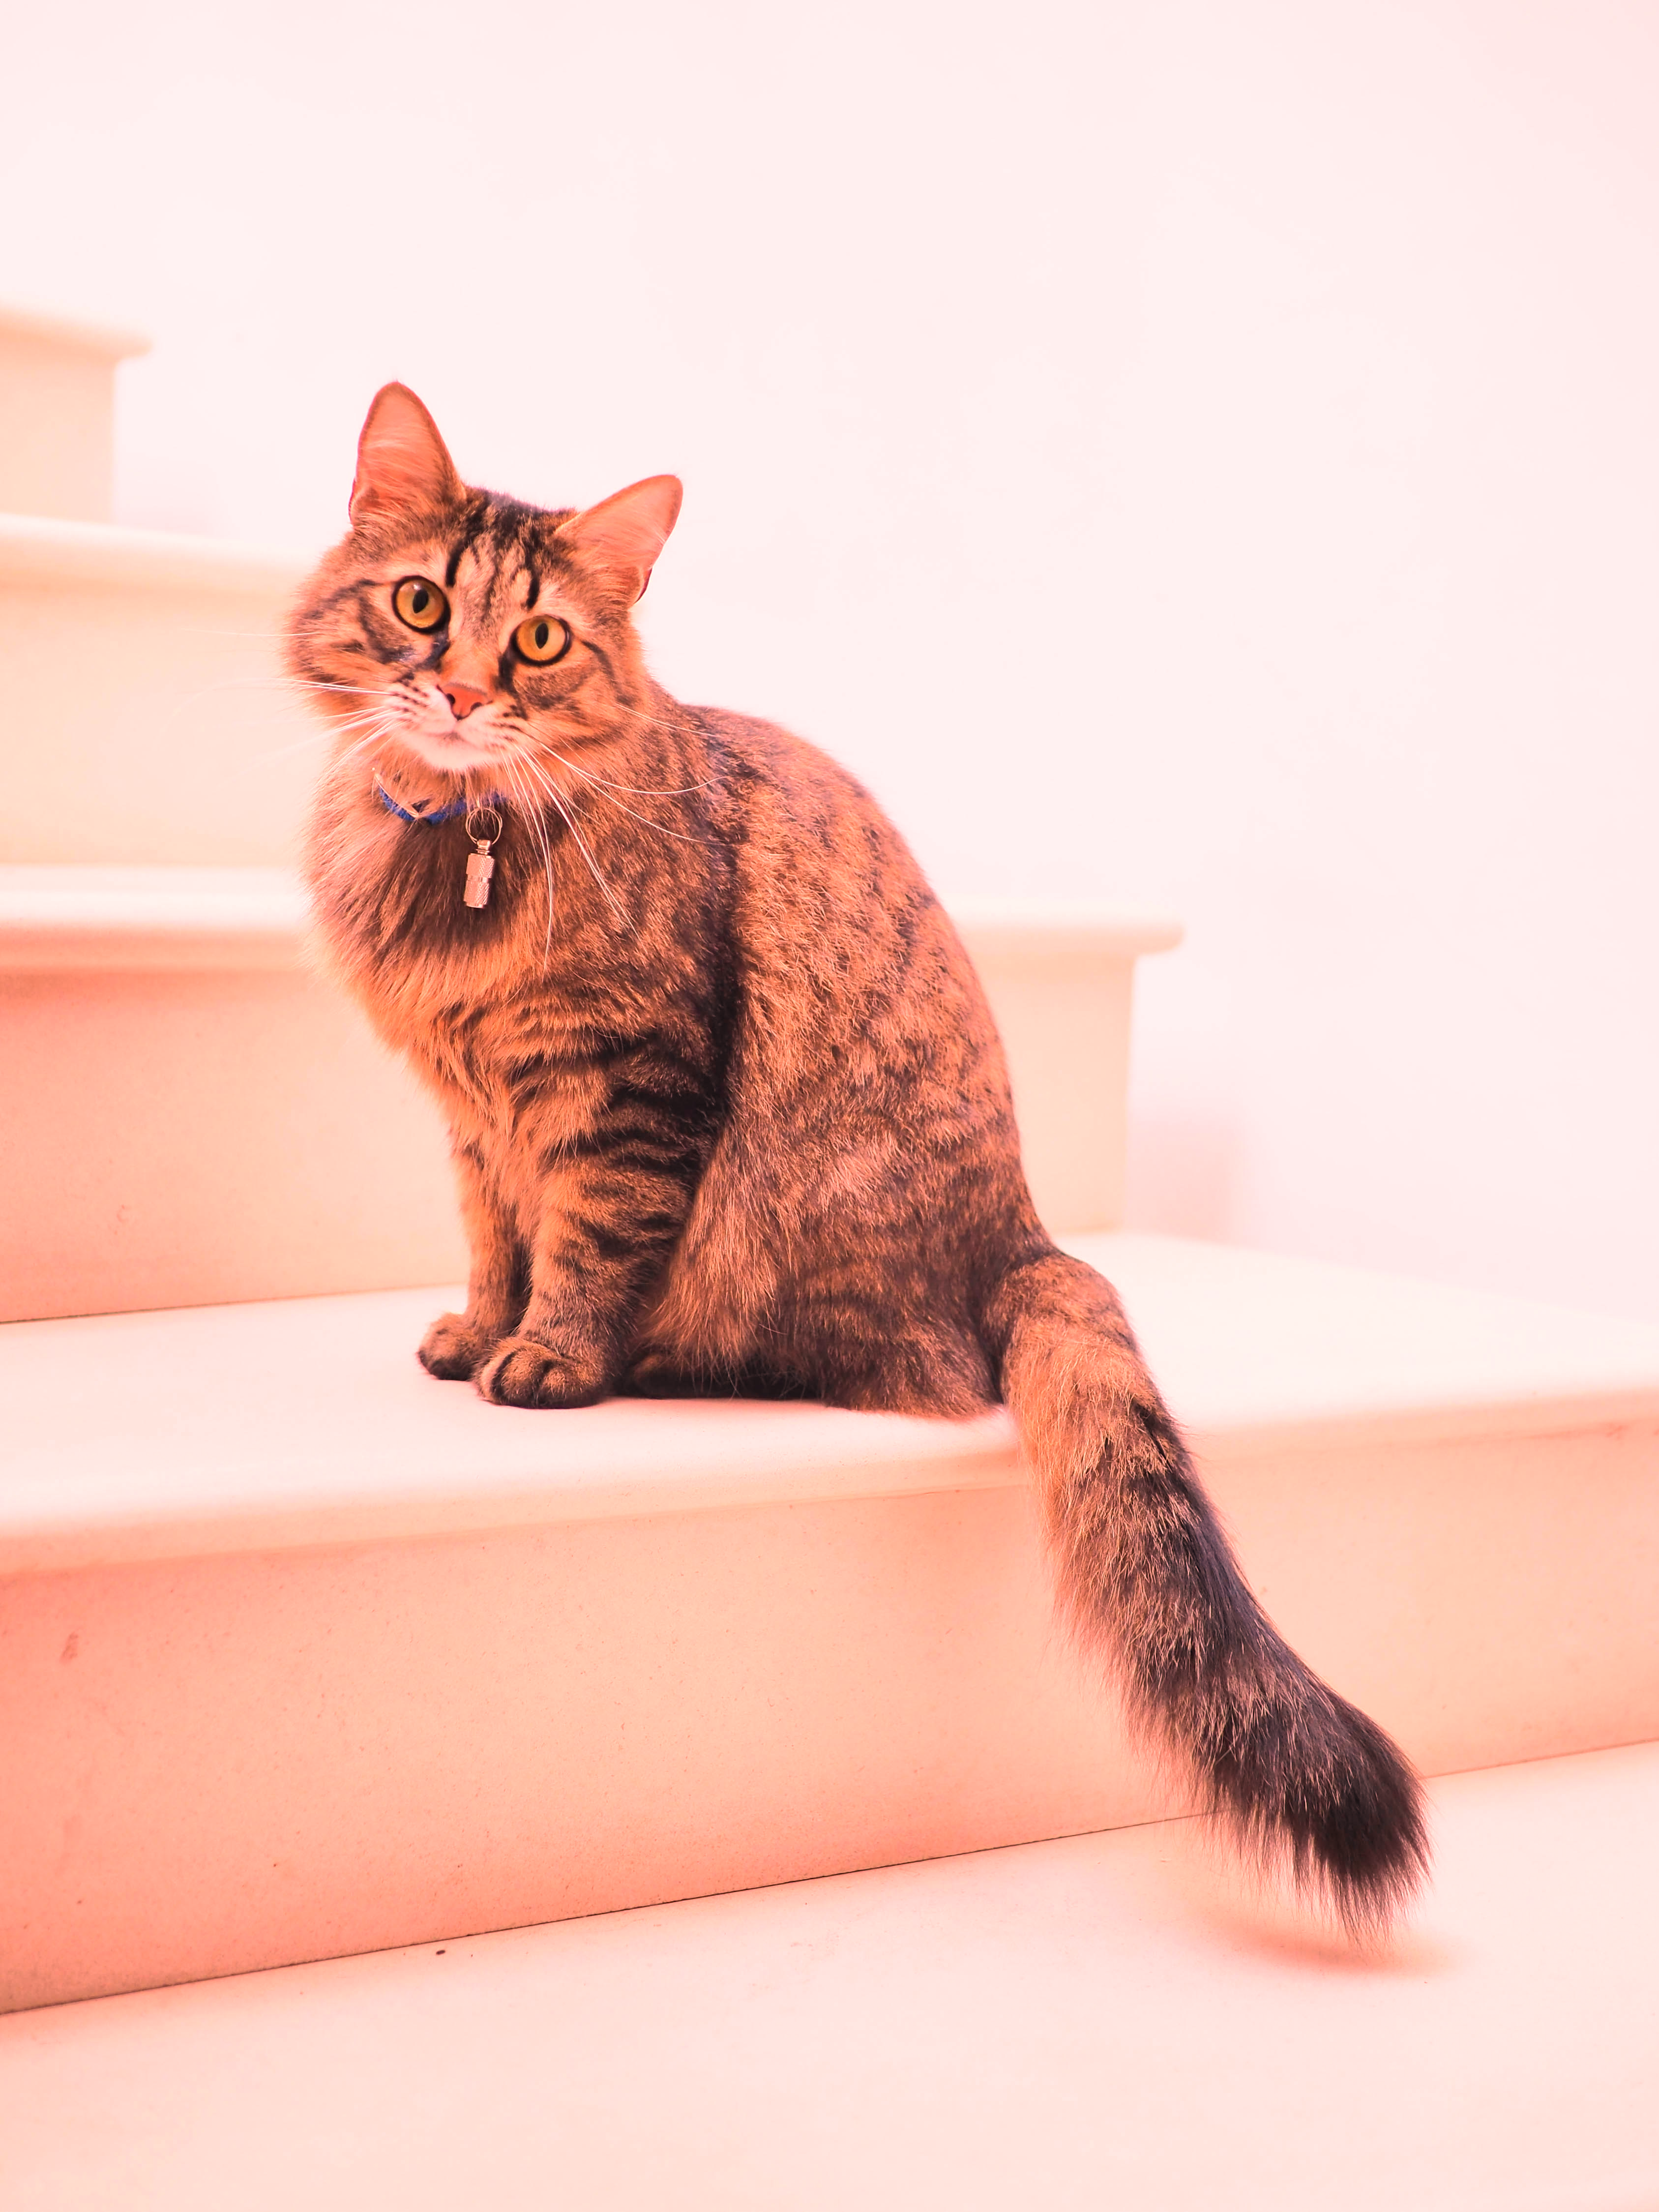
\includegraphics[width=0.5\textwidth]{report_images/task4_enhanced.png}
    \caption{Enhanced Image (Red Channel +50\%)}
\end{figure}

\subsection{Observation}
Enhancing a specific channel increases its intensity relative to others, giving the image a tint of that color.

\section{Task 5: Grayscale Image Negation}

\subsection{Problem Statement}
Create a function to compute the negative of a grayscale image using the formula:
\[ g(x, y) = L_{max} - f(x, y) \]
where $L_{max} = 255$ for 8-bit images.

\subsection{Solution Approach}
Each pixel intensity is subtracted from 255. This inverts the brightness, making dark areas light and light areas dark.

\subsection{Implementation}
\begin{lstlisting}[language=Python]
def grayscale_negative(gray_img):
    Lmax = 255
    negative_img = Lmax - gray_img
    cv2_imshow(negative_img)
    return negative_img
\end{lstlisting}

\subsection{Output}
The negative of the grayscale image is shown below.

\begin{figure}[H]
    \centering
    \includegraphics[width=0.5\textwidth]{report_images/task5_negative_gray.png}
    \caption{Negative Grayscale Image}
\end{figure}

\subsection{Observation}
Inverting pixel values transforms light regions to dark and vice versa, effectively creating a photographic negative.

\section{Task 6: Color Image Negation}

\subsection{Problem Statement}
Extend the grayscale negation function to work with color images.

\subsection{Solution Approach}
The negation operation is applied to the color image. Since NumPy operations are element-wise, subtracting the image array from 255 inverts all three channels (R, G, B) simultaneously.

\subsection{Implementation}
\begin{lstlisting}[language=Python]
def invert_color(color_image):
    negative_img = 255 - color_image
    cv2_imshow(negative_img)
    return negative_img
\end{lstlisting}

\subsection{Output}
The negative of the color image is shown below.

\begin{figure}[H]
    \centering
    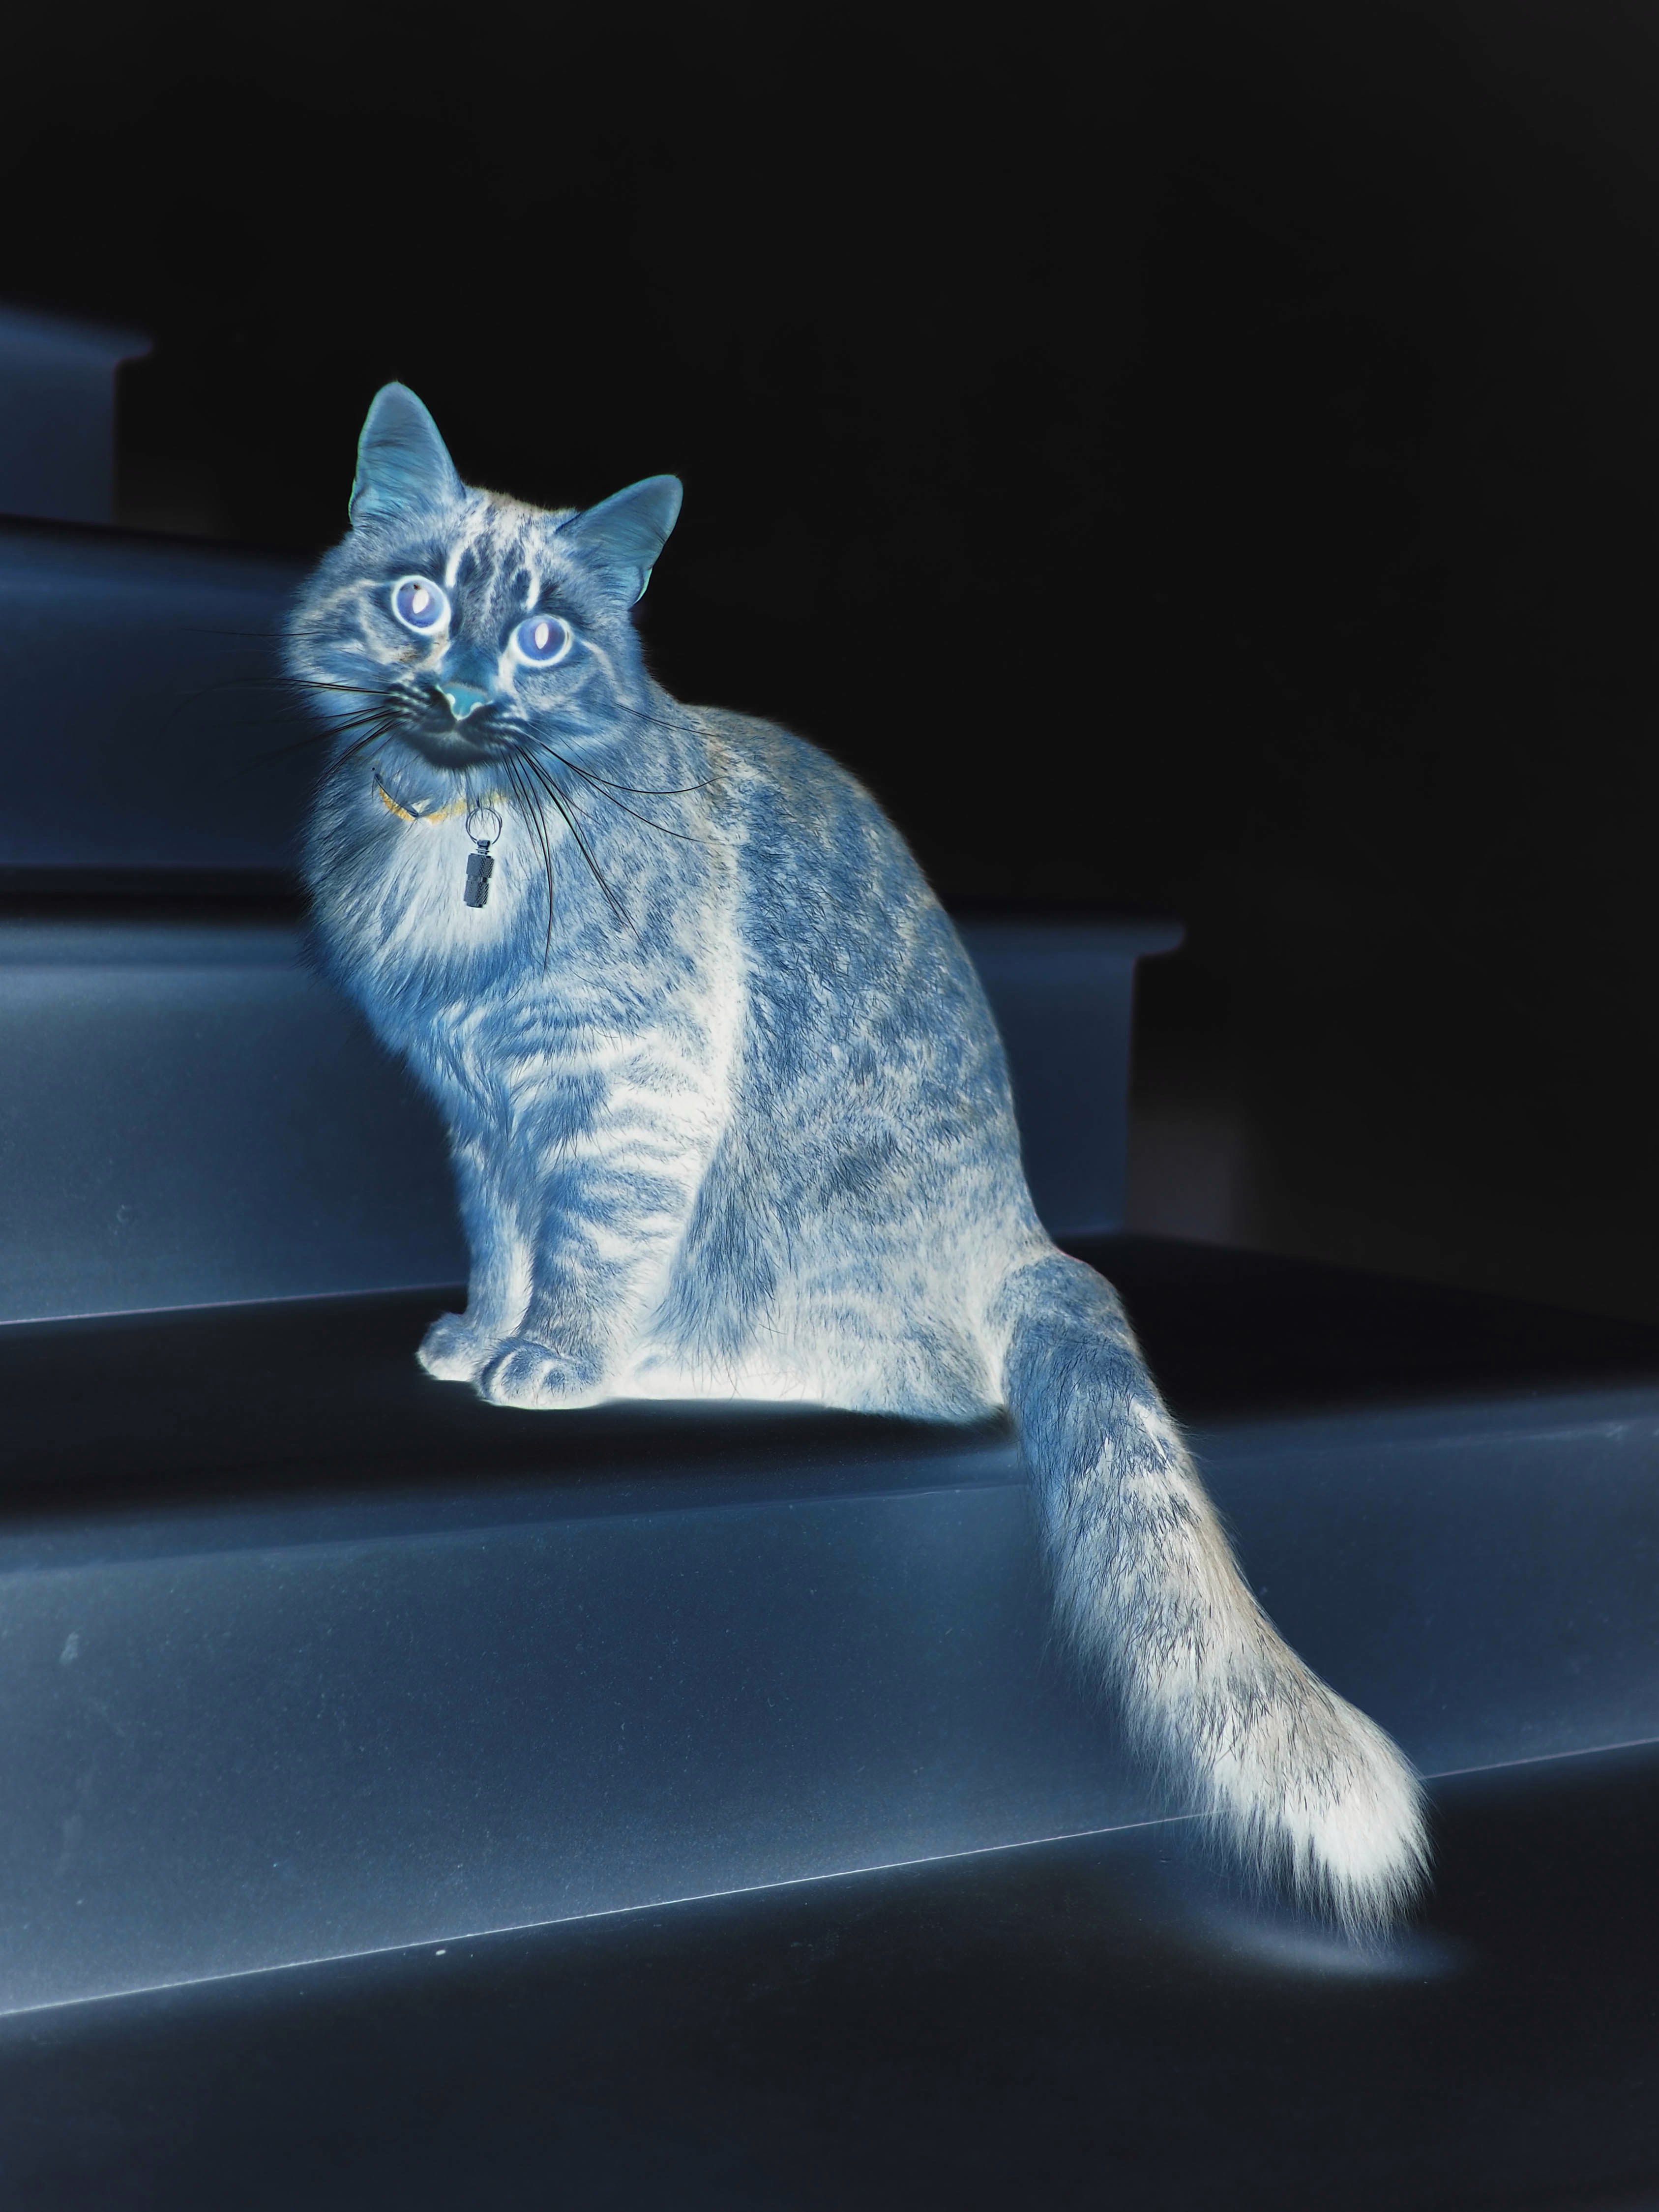
\includegraphics[width=0.5\textwidth]{report_images/task6_negative_color.png}
    \caption{Negative Color Image}
\end{figure}

\subsection{Observation}
Inverting color channels produces complementary colors, where red becomes cyan, green becomes magenta, and blue becomes yellow.

\end{document}
